
In applied phylogenetics it rarely happens that trees are binary. Often there is insufficient information available to be able to determine the exact order in which several branching events occurred, and it is standard practice to model this uncertainty using vertices with outdegree higher than two: a \emph{soft polytomy} \cite{davidbook}. Hence it is important to develop algorithms for the \emph{nonbinary} case i.e., when the trees are not necessarily binary and high-degree vertices capture a set of equally likely branching scenarios. 


As was the case in the binary setting, the problem \maaf is NP-hard and APX-hard \cite{bordewich07a}. In the previous chapter we showed how, for the binary variant of \maaf, large instances \emph{can} however be very well approximated using a specific marriage of \maf and \dfvs solvers. This approach is exponential-time in the worst case but in practice is very fast and yields highly competitive approximation factors. %The question remained whether a similar approach would work for \emph{nonbinary} \maaf.

In this chapter we give three algorithms for nonbinary agreement forests. We start with a polynomial-time 4-approximation for \maf on two nonbinary trees. Proving its correctness almost immediately led to an $O(4^k \text{poly}(n))$ time exact algorithm for the same problem. This is presented in Section \ref{sec:nbmaf}. As promised in the previous chapter, we then move on to show that a $c$-approximation algorithm for nonbinary \maf and a $d$-approximation algorithm for \dfvs can be combined to yield a $d(c+3)$-approximation for nonbinary \maaf in Section \ref{sec:nbmaaf}. Combining this with our polynomial-time 4-approximation for \maf, we obtain a 7$d$-approximation for \maaf. As we discuss in the conclusion, it is likely that in practice $d=1$ can be obtained using ILP to solve the generated \dfvs instances. Hence, using the 4-approximation for nonbinary \maf we get an exponential-time 7-approximation for nonbinary \maaf and using the FPT algorithm for nonbinary \maf we get an exponential-time 4-approximation for nonbinary \maaf. If we wish a purely polynomial-time approximation, we can use the best-known polynomial-time approximation algorithm for \dfvs, yielding overall a polynomial-time $O(\log(k)\log(\log(k)))$-approximation for nonbinary \maaf, with~$k$ the size of a maximum acyclic agreement forest minus one. 
%We mention here that our algorithms for \maf are partly based on the ideas in~\cite{whiddenFixed} and the algorithm for \maaf on the ideas in~\cite{practicalCycleKiller} but the analysis is different in both cases because nonbinary agreement forests are substantially different from binary agreement forests. In fact, high-outdegree vertices pose a formidable challenge because of the freedom to refine these vertices in one of exponentially many ways.

\begin{figure}
    \centering
    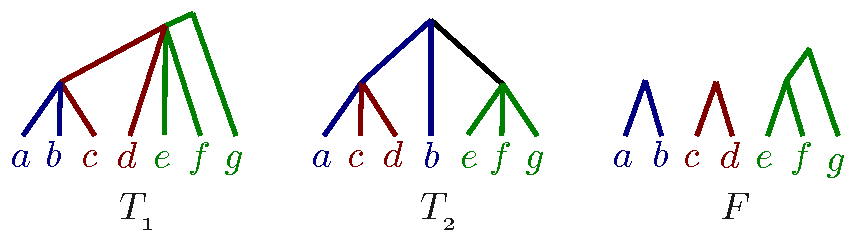
\includegraphics[scale=.8]{../figs/fig_maf2}
    \caption{Two nonbinary rooted phylogenetic trees~$T_1$ and~$T_2$ and a maximum agreement forest~$F$ of~$T_1$ and~$T_2$.\label{fig:maf}}
\end{figure}

We start by giving definitions for the nonbinary versions of the concepts we have already encountered in the introduction and previous chapters. Recall that \emph{forest} is defined as a set of trees. To avoid confusion, we call each element of a forest a \emph{component}, rather than a tree. Let~$T$ be a tree and~$\cF$ a forest. We say that~$\cF$ is a \emph{forest for}~$T$ if:
\begin{itemize}
\item each component~$F\in\cF$ is a refinement of $T|L(F)$;
\item the subtrees $\{T(L(F))\mid F\in \cF\}$ are edge-disjoint; and
\item the union of $L(F)$ over all $F\in \cF$ is equal to~$L(T)$.
\end{itemize}

By this definition, if~$\cF$ is a forest for some tree~$T$, then $\{L(F)\mid F\in\cF\}$ is a partition of the leaf set of~$T$. It will indeed sometimes be useful to see an agreement forest as a partition of the leaves, and sometimes to see it as a collection of trees.

If~$T_1$ and~$T_2$ are two trees, then a forest~$\cF$ is an \emph{agreement forest} of~$T_1$ and~$T_2$ if it is a forest for~$T_1$ and a forest for~$T_2$. The \emph{size} of a forest~$\cF$, denoted by~$|\cF|$, is defined as the number of its components. We consider the following computational problem. \\

\noindent{\bf Problem:} {\sc Nonbinary Maximum Agreement Forest} (Nonbinary \maf)\\
\noindent {\bf Instance:} Two rooted phylogenetic trees~$T_1$ and~$T_2$. \\
\noindent {\bf Solution:} An agreement forest~$\cF$ of~$T_1$ and~$T_2$.\\
\noindent {\bf Objective:} Minimize~$|\cF|-1$.\\

We define the \emph{inheritance graph} $IG(T_1,T_2,\cF)$ of an agreement forest, as the directed graph whose vertices are the components of~$\cF$ and which has an edge~$(F,F')$ precisely if either
\begin{itemize}
\item there exists a path in~$T_1$ from the root of $T_1(L(F))$ to the root of $T_1(L(F'))$ containing an edge of $T_1(L(F))$ or;
\item there exists a path in~$T_2$ from the root of $T_2(L(F))$ to the root of $T_2(L(F'))$ containing an edge of $T_2(L(F))$.
\end{itemize}

Note that if there exists a path in~$T_i$ (for $i\in\{1,2\}$) from the root of $T_i(L(F))$ to the root of $T_i(L(F'))$ containing an edge of $T_i(L(F))$, then this directly implies that this path also contains such an edge that has the root of $T_i(L(F))$ as tail.

An agreement forest~$\cF$ of~$T_1$ and~$T_2$ is called an \emph{acyclic agreement forest} if the graph $IG(T_1,T_2,\cF)$ is acyclic.

We call a forest an {\em $\cF$-splitting} if it is an acyclic agreement forest that can be obtained from a refinement of~$\cF$ by removing edges and suppressing vertices with in- and outdegree~1.

A \emph{maximum acyclic agreement forest} (\maaf) of~$T_1$ and~$T_2$ is an acyclic agreement forest of~$T_1$ and~$T_2$ with a minimum number of components. \\

\noindent{\bf Problem:} {\sc Nonbinary Maximum Acyclic Agreement Forest} (Nonbinary \maaf)\\
\noindent {\bf Instance:} Two rooted phylogenetic trees~$T_1$ and~$T_2$. \\
\noindent {\bf Solution:} An acyclic agreement forest~$\cF$ of~$T_1$ and~$T_2$.\\
\noindent {\bf Objective:} Minimize~$|\cF|-1$.\\

We use the notation \maf$(T_1,T_2)$ and \maaf$(T_1,T_2)$ for the optimal objective value of, respectively, a maximum agreement forest and a maximum acyclic agreement forest for input trees~$T_1$ and~$T_2$. Hence, if~$\cA$ is a maximum agreement forest and~$\cM$ is a maximum acyclic agreement forest, then \maf$(T_1,T_2)=|\cA|-1$ and \maaf$(T_1,T_2)=|\cM|-1$.



%
%The \maaf problem is closely related to an important problem in phylogenetics. Using~$\delta^-(v)$ to denote the indegree of a vertex~$v$, a \emph{reticulation} is a vertex~$v$ with~$\delta^-(v)\geq 2$. The \emph{reticulation number} of a network~$N$ is given by
%
%\[
%r(N)=\sum_{v: \delta^-(v)\geq 2}(\delta^-(v)-1).
%\]
%
%In \cite{baroni05} it was shown that, in the binary case, the optimum to {\sc maaf} is equal to the optimum of the following problem. Later, in \cite{linzsemple2009}, this characterisation
%was extended to nonbinary trees.
%
%\noindent{\bf Problem:} {\sc Nonbinary Minimum Hybridization} (Nonbinary \textsc{mh})\\
%\noindent {\bf Instance:} Two rooted phylogenetic trees $T_1$ and $T_2$. \\
%\noindent {\bf Solution:} A phylogenetic network~$N$ that displays $T_1$ and $T_2$.\\
%\noindent {\bf Objective:} Minimize~$r(N)$.\\
%
%Moreover, it was shown that, for two trees~$T_1,T_2$, \emph{any} acyclic agreement forest for~$T_1$ and~$T_2$ with~$k+1$ components can be turned into a phylogenetic network that displays~$T_1$ and~$T_2$ and has reticulation number~$k$, and vice versa. Thus, any approximation for Nonbinary \maaf gives an approximation for nonbinary {\sc {mh}}.
%
%There is also a less obvious relation between \maaf and the \emph{directed feedback vertex set problem}, a problem which is well-known in the communities of theoretical computer science and combinatorial optimisation. A feedback vertex set of a directed graph is a subset of the vertices that contains at least one vertex of each directed cycle. Equivalently, a subset of the vertices of a directed graph is a \emph{feedback vertex set} if removing these vertices from the graph makes it acyclic.\\
%
%\noindent{\bf Problem:} Directed Feedback Vertex Set (\dfvs)\\
%\noindent {\bf Instance:} A directed graph~$D$. \\
%\noindent {\bf Solution:} A feedback vertex set~$S$ of $D$. \\
%\noindent {\bf Objective:} Minimize~$|S|$.\\ 


\section{Nonbinary \maf}
\label{sec:nbmaf}

In the first part of this section we present a 4-approximation algorithm for \maf and prove the following theorem:

\begin{theorem}\label{thm:maf}
There is a polynomial-time 4-approximation for (nonbinary) \maf.
\end{theorem}

The performance analysis leads almost straightforwardly to a fixed parameter tractability result, which we present in the second part as this theorem.

\begin{theorem}\label{thm:fpt}
Nonbinary \maf can be solved exactly in $O(4^k \text{poly}(n))$ time, with~$n$ the number of leaves and~$k$ the number of components of a maximum agreement forest minus one.
\end{theorem}

\subsection*{Approximation of nonbinary \maf}


Let~$T_1$ and~$T_2$ be the input trees to \maf. They do not have to be binary. We will construct a forest by {iteratively ``cutting''~$T_2$ and collapsing leaves of~$T_1$ and~$T_2$}. A ``cut'' operation of $T_2$ consists of removing an edge (and suppressing indegree-1 outdegree-1 vertices) or of first refining a vertex (with outdegree greater than~2) and then removing an edge (and suppressing indegree-1 outdegree-1 vertices), see Figure~\ref{fig:cut}.

\begin{figure}
\centering
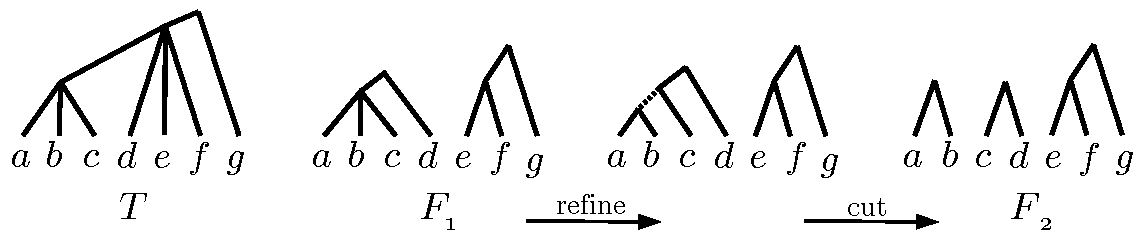
\includegraphics[scale=.8]{../figs/fig_cut}
\caption{A tree~$T$ and two forests~$F_1$ and~$F_2$ for~$T$. Forest~$F_2$ can be obtained from~$F_1$ by refining the parent of~$a,b$ and~$c$ and subsequently removing an edge and suppressing an indegree-1 outdegree-1 vertex.\label{fig:cut}}
\end{figure}

Let~$F_2$ be the forest obtained by cutting~$T_2$ {in a particular iteration}. In each iteration, we further cut~$F_2$ until at some point~$F_2$ becomes a forest also of~$T_1$. At that point, we have successfully obtained an agreement forest for~$T_1$ and~$T_2$ and we terminate the algorithm.

We describe an algorithm to determine which edges to cut by defining an iteration of the algorithm. Suppose that at the start of the iteration we have an (intermediate) forest~$F_2$. There are two main cases. In each case, the algorithm will make at most~4 cuts, and we will show that at least one of these cuts is unavoidable, thus showing that in each case a 4-approximation is attained.

Take an arbitrary internal vertex~$u$ of {a reduced}~$T_1$ with the property that all its children are leaves. Such a vertex clearly exists in any tree. Let~$C$ be the set of children of~$u$ in~$T_1$ and~$\bar{C}$ the set of all leaves that are not in~$C$.

First the algorithm checks the following three simple cases in the given order.

\smallskip

\noindent {\bf Case 0a.} There exist $c_1,c_2\in C$ that have a common parent in~$F_2$.

In this case, we collapse the subtree on $c_1$ and~$c_2$ to a single leaf in both~$T_1$ and~$F_2$. To be precise, we do the following in both~$T_1$ and~$F_2$. If~$c_1$ and~$c_2$ have no siblings, we delete~$c_1$ and~$c_2$ and label their former parent by~$\{c_1,c_2\}$. If~$c_1$ and~$c_2$ do have siblings, we delete~$c_1$ and replace label~$c_2$ by label~$\{c_1,c_2\}$.

\smallskip

\noindent {\bf Case 0b.} Some leaf~$c\in C$ is an isolated vertex in~$F_2$.

In this case, we remove~$c$ from both~$T_1$ and~$F_2$ and suppress any resulting outdegree-1 vertices. At the end, after recursively having computed an agreement forest, we add an isolated vertex for~$c$.

\smallskip

\noindent {\bf Case 0c.} The leaves in~$C$ are all in different components of~$F_2$. 

In this case, we remove all~$c\in C$ from both~$T_1$ and~$F_2$ and suppress any resulting outdegree-1 vertices. At the end, after recursively having computed an agreement forest, we add isolated vertices for all~$c\in C$.

\smallskip

Correctness of the procedure followed in the first two cases is obvious. To prove correctness in Case~0c, let~$F$ be an agreement forest of~$T_1$ and~$T_2$ that can be obtained by cutting~$F_2$. Since the leaves in~$C$ are all in different components of~$F_2$, they are all in different components of~$F$. Observe that any component of~$F$ that contains an element of~$C$ and an element of~$\bar{C}$ has to use the edge entering~$u$ in~$T_1$. It follows that at most one component of~$F$ contains an element of~$C$ and an element of~$\bar{C}$. Since the elements of~$C$ are all in different components of~$F$, it follows that at most one element from~$C$ is \emph{not} a singleton in~$F$. Hence, at most one of the cuts made in this step is avoidable. At least~2 cuts were made because $|C|\geq 2$ and no~$c\in C$ was already an isolated vertex in~$F_2$ by Case 0b. It follows that at least half of the cuts made were unavoidable.

If none of the above cases applies, the algorithm picks~$c_1,c_2$ from~$C$ in such a way that~$c_1$ and~$c_2$ are in the same component~$A_2$ of~$F_2$ and such that their lowest common ancestor in~$A_2$ is at maximum distance from the root of the component. Moreover, if there exists such a pair for which neither of~$c_1$ and~$c_2$ is a child of their lowest common ancestor, we pick such a pair first.

\smallskip

\noindent {\bf Case 1.} Neither of~$c_1$ and~$c_2$ is a child of their lowest common ancestor~$v$ in~$F_2$.

Let~$p_1$ be the parent of~$c_1$ and~$p_2$ the parent of~$c_2$ in~$F_2$. (We have $p_1\neq p_2$ because we are not in Case 0a, {but also because otherwise the lowest common ancestor of $v$ would be $p_1= p_2$}.) Let~$S_1$ be the set of all leaves that are descendants of~$p_1$ except for~$c_1$. Similarly, let~$S_2$ be the set of all leaves that are descendants of~$p_2$ except for~$c_2$. Finally, let~$R$ be the set of other leaves of component $A_2$, i.e. leaves that are not in $S_1\cup S_2\cup\{c_1,c_2\}$. We cut~$A_2$ by creating separate components for~$c_1,c_2,S_1,S_2$ and~$R$, thus making four cuts, see Figure~\ref{fig:case1}.

\begin{figure}
    \centering
    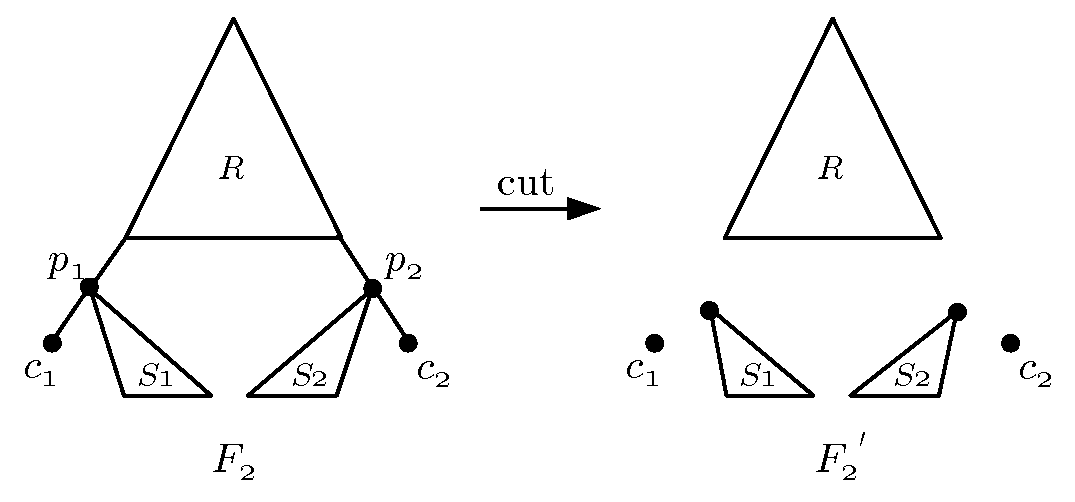
\includegraphics[scale=.7]{../figs/fig_case1}
    \caption{Case 1: none of~$c_1$ and~$c_2$ is a child of their lowest common ancestor. We cut~$F_2$ into~$F_2'$ by creating separate components for~$c_1,c_2,S_1,S_2$ and~$R$.\label{fig:case1}
    }
\end{figure}

We claim that at least one of these four cuts was unavoidable. Let~$F$ be an agreement forest of~$T_1$ and~$T_2$ with a minimum number of components. If any of~$c_1,c_2$ is a singleton in~$F$, then the cut that removed the edge entering that vertex was unavoidable. Hence, we assume that~$c_1$ and~$c_2$ are both non-singletons in~$F$. Suppose~$c_1$ and~$c_2$ are in the same component of~$F$. Because of the choice of~$c_1$ and~$c_2$ having their lowest common ancestor furthest from the root of the component,~$S_1,S_2\subset \bar{C}$; they contain no element of~$C$. Hence cutting off both $S_1$ and $S_2$ is unavoidable.

Hence, we assume that~$c_1$ and~$c_2$ are in different, non-singleton components of~$F$. As argued before, in justifying Case~0c, at most one of~$c_1$ and~$c_2$ can be in a component with elements from~$\bar{C}$. Moreover, as also argued before, $S_1,S_2\subset \bar{C}$. Therefore, at most one of~$c_1$ and~$c_2$ can be in a component with elements from $S_1\cup S_2$. W.l.o.g. suppose $c_1$ is not in a component with elements from $S_1\cup S_2$. Since~$c_1$ is not a singleton component, it is contained in a component which uses the edge of~$A_2$ entering~$p_1$ and the edge from~$p_1$ to~$c_1$, but none of the other edges leaving~$p_1$. Hence, the cut cutting off~$S_1$ is unavoidable. Similarly, if~$c_2$ is not in a component with elements from $S_1\cup S_2$, then the cut cutting off~$S_2$ is unavoidable. Thus, always at least one of the four cuts was unavoidable.

\smallskip

\noindent {\bf Case 2.} Either $c_1$ or $c_2$ is a child of their lowest common ancestor~$v$ in~$F_2$. 

Let~$c_1,c_2$ be any such pair. Let again~$p_1$ be the parent of~$c_1$ and~$p_2$ the parent of~$c_2$ in~$F_2$. Assume without loss of generality that~$p_1$ is the lowest common ancestor of~$c_1$ and~$c_2$. Let~$S_2$ contain all leaves that are descendants of~$p_2$ except for~$c_2$. Let~$S_1$ contain all leaves that are descendants of~$p_1$ except for $c_1,c_2$ and the leaves in~$S_2$. Let~$R$ contain all remaining leaves. We cut~$F_2$ by creating separate components for~$c_1,c_2,S_1,S_2$ and~$R$, thus making four cuts, see Figure~\ref{fig:case2}.

\begin{figure}
    \centering
    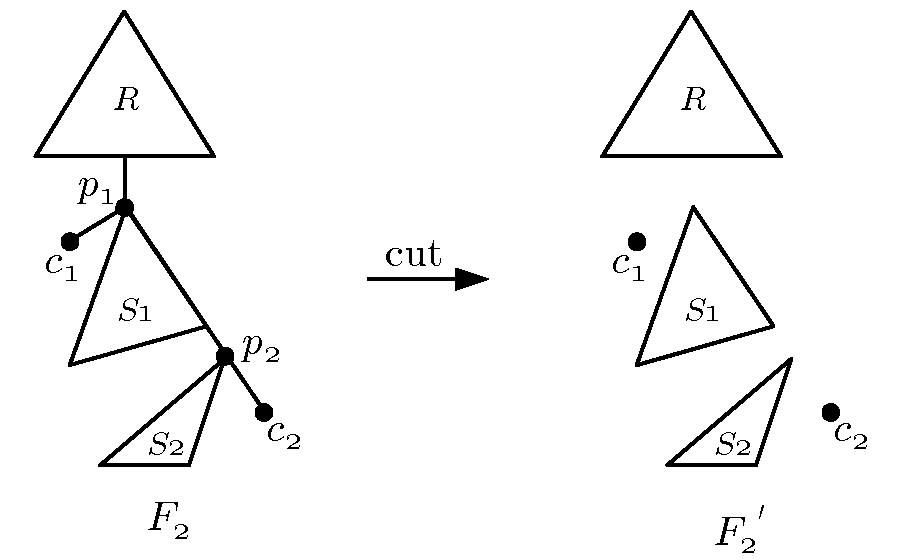
\includegraphics[scale=.7]{../figs/fig_case2}
    \caption{Case 2: $c_1$ is a child of the lowest common ancestor of~$c_1$ and~$c_2$. We cut~$F_2$ into~$F_2'$ by creating separate components for~$c_1,c_2,S_1,S_2$ and~$R$.
    \label{fig:case2}}
\end{figure}

We claim that also in this case at least one of the four cuts was unavoidable. Let~$F$ again be an agreement forest of~$T_1$ and~$T_2$ with a minimum number of components. We can argue as before that we can restrict attention to the situation in which~$c_1$ and~$c_2$ are non-singletons and belong to different components. It is also again true that~$S_1$ and~$S_2$ cannot contain elements from~$C$. To see this, first note that no element~$c_3$ of~$C\setminus\{c_1\}$ can be a child of~$p_1$ because then~$c_1,c_3\in C$ would have a common parent in~$F_2$, which is a Case~0a situation. Moreover, no~$c_3\in C\setminus\{c_1,c_2\}$ can be reached from~$p_1$ by a directed path with at least one internal vertex that does not belong to the path from $p_1$ to~$c_2$, because then $c_2,c_3$ would conform to Case~1. Finally, as before, no~$c_3\in C\setminus\{c_1,c_2\}$ can be reached from an internal vertex of the path from~$p_1$ to~$c_2$ because then~$c_3$ and~$c_2$ would have a lowest common ancestor further away from the root than~$p_1$. We conclude that~$S_1$ and~$S_2$ contain no elements from~$C$.

As in Case~1, it follows that at most one of~$c_1$ and~$c_2$ is in a component with elements from~$S_1\cup S_2$. Also, similar to the arguments in Case 1, if $c_1$ is not in a component with elements from~$S_1\cup S_2$ then that component uses the edge of~$A_2$ entering~$p_1$ and the edge from~$p_1$ to~$c_1$, but no other edges leaving~$p_1$. Hence, the cutting off $S_1\cup S_2\cup \{c_2\}$ is unavoidable. If~$c_2$ is not in a component with elements from~$S_1\cup S_2$, then cutting off~$S_2$ is unavoidable.

Hence, we conclude that in each case at least one of the four cuts is unavoidable, and the algorithm thus yields a 4-approximation.

\subsection*{An FPT algorithm for nonbinary \maf}

In this section, we show that there exists an $O(4^k \text{poly}(n))$ time algorithm for nonbinary \maf, i.e., we prove Theorem~\ref{thm:fpt}.

The algorithm follows the same ideas as the approximation algorithm in the proof of Theorem~\ref{thm:maf}. Cases~0a and 0b are executed in exactly the same way. In Case 0c, instead of removing all~$c\in C$, we pick~$c_1,c_2\in C$ arbitrarily and branch into two subproblems. In one subproblem~$c_1$ is removed and in the other subproblem~$c_2$ is removed. After recursively computing an agreement forest, the removed leaf is added as an isolated vertex. This step is correct since, by the proof of Theorem~\ref{thm:maf}, in any maximum agreement forest at least one of~$c_1$ and~$c_2$ is an isolated vertex. For Cases~1 and~2, instead of making four cuts, we branch into four subproblems, one for each possible cut. By the proof of Theorem~\ref{thm:maf}, at least one of the four cuts is unavoidable, and hence at least one subproblem has the same optimum as the original problem.

It remains to analyze the running time. In each step we branch into at most four subproblems. For each subproblem we make one cut, and hence we reduce the parameter~$k$ by one. Therefore, at most~$4^k$ subproblems are created. For each subproblem, we need only time polynomial in~$n$. This concludes the proof.





\section{Approximating nonbinary \maaf}
\label{sec:nbmaaf}


In this section we relate approximability of Nonbinary \maaf to that of Nonbinary \maf and \dfvs and prove the following theorem:

\begin{theorem}
\label{thm:maafapprox}
If there exists a $c$-approximation for Nonbinary \maf and a $d$-approximation for \dfvs, then there exists a $d(c+3)$-approximation for Nonbinary \maaf and hence for Nonbinary \mh.
\end{theorem}


Combining this Theorem with a Theorem~\ref{thm:maf} from the previous section, we obtain the following corollary.

\begin{corollary}
If there exists a $d$-approximation for \dfvs then there exists a $7d$-approximation for Nonbinary \maaf and hence for Nonbinary \mh.
\end{corollary}

Moreover, using the $O(\log(\tau)\log(\log(\tau)))$-approximation for weighted \dfvs from~\cite{dfvsApprox}, with~$\tau$ the weight of a minimum feedback vertex set, we also obtain the following.

\begin{corollary}
There exists a polynomial-time $O(\log(k)\log(\log(k)))$-approximation for nonbinary \maaf, with~$k$ the number of components of a maximum acyclic agreement forest minus one.
\end{corollary}


%\textcolor{red}{TO DO: go through the proof of this section and indicate where the c+3 comes from instead of c+1 which was the case for binary trees. I used to know this very clearly, should still be possible to find and explain the intuition.}

An agreement forest~$\cA$ is said to be \emph{maximal} if there is no agreement forest that can be obtained from~$\cA$ by merging components. It is clear that, given any agreement forest, a maximal agreement forest with at most as many components can be obtained in polynomial time.

Let~$T_1$ and~$T_2$ be two nonbinary trees. Consider a maximal agreement forest~$\cA$ and let~$\cM$ be some maximum acyclic agreement forest for these two trees. We will first prove that there exists an $\cA$-splitting of size at most $|\cA|+3|\cM|$. After that, we will show how the problem of finding an optimal $\cA$-splitting can be reduced to \dfvs.

The idea of the first part of the proof is to split components of~$\cA$ according to~$\cM$. We show that to make~$\cA$ acyclic we will increase the number of components of~$\cA$ by at most three times the size of~$\cM$.

We start with some definitions. In the first part of the proof, we see an agreement forest~$\cA$ for~$T_1$ and~$T_2$ as a partition of the leaf set~$X$ for which holds that:
\begin{enumerate}
\item $T_1|A$ and~$T_2|A$ have a common refinement, for all~$A\in\cA$; and
\item the subtrees $\{T_i(A)\mid A\in\cA\}$ are edge-disjoint, for~$i\in\{1,2\}$.
\end{enumerate}

Using this definition of agreement forests, an $\cA$-splitting is an acyclic agreement forest that can be obtained by splitting components of~$\cA$. The following observation is easily verifiable.

\begin{observation}\label{obs:acylic}
If~$\cM$ is an acyclic agreement forest and~$\cM'$ is an agreement forest that can be obtained from~$\cM$ by splitting components, then~$\cM'$ is an acyclic agreement forest.
\end{observation}

For a component~$A$ of an agreement forest for two trees~$T_1$ and~$T_2$, we write $r_i(A)$ to denote the root of $T_i(A)$, for~$i\in\{1,2\}$. For two components~$M$ and~$M'$ of~$\cM$, we say that~$M$ is \emph{lower} than~$M'$ if in the inheritance graph of~$\cM$ there is a directed path (and hence an edge) from~$M'$ to~$M$. Since the inheritance graph of~$\cM$ is acyclic,~$\cM$ contains some lowest element. Moreover, for any subset of components of~$\cM$, there exists a component that is lowest over that subset. For a component~$A$ of~$\cA$ and a component~$M$ of~$\cM$, we say that~$M$ {\em properly intersects}~$A$ (and that~$A$ is~\emph{properly intersected by}~$M$) if $M\cap A \neq \emptyset$ and $A\setminus M\neq \emptyset$.

We are now ready to describe the procedure for splitting~$\cA$. Initially, all components of~$\cA$ and~$\cM$ are unmarked. We iteratively choose a component~$M^*$ of~$\cM$ that is lowest over all unmarked components of~$\cM$. For each component~$A$ of~$\cA$ that is properly intersected by~$M^*$, we split~$A$ into two components $A\cap M^*$ and $A\setminus M^*$ and we mark $A\cap M^*$. Then we mark~$M^*$ and any unmarked components~$A'$ of~$\cA$ with $A'\subseteq M^*$ and proceed to the next iteration. We continue this procedure until all components of~$\cM$ are marked.

It is clear that, if~$\cA^*$ is the agreement forest obtained at the end of some iteration, then no marked component of~$\cM$ properly intersects any component of~$\cA^*$. Moreover, no marked component of~$\cA^*$ is properly intersected by any component of~$\cM$.

\begin{lemma}
\label{lem:edgedisjoint}
Let~$\cA$ be an agreement forest for~$T_1$ and~$T_2$, let~$M^*$ be a component of~$\cM$ that is lowest over all unmarked components of~$\cM$ and let~$A$ be a component of~$\cA$ that is properly intersected by~$M^*$. Then, $T_i(A \cap M^*)$ and $T_i(A\setminus M^*)$ are edge-disjoint subtrees of~$T_i$, for $i\in\{1,2\}$.
\end{lemma}
\begin{proof}
Suppose to the contrary that in at least one tree, say~$T_1$, there exists an edge~$e$ such that $e\in T_1(A \cap M^*)$ and $e\in T_1(A\setminus M^*)$. Consider the set of leaves~$S$ that can be reached from~$e$. Clearly, some leaf of $A\setminus M^*$ has to be in~$S$. Let $x\in S \cap (A\setminus M^*)$. Clearly,~$x$ must be in some component of~$\cM$ other than~$M^*$. Call that component~$M'$. Since components of~$\cM$ are edge disjoint, $r_1(M')$ has to be below~$e$. Because $e\in T_1(A \cap M^*)$, it follows that $e\in T_1(M^*)$ and hence that~$M'$ is lower than~$M^*$. Since $M^*$ is lowest over all unmarked components of~$\cM$, it follows that~$M'$ is marked and hence that~$M'$ does not properly intersect any component of~$\cA$. This is a contradiction because~$M'$ properly intersects~$A$.
\end{proof}

Lemma \ref{lem:edgedisjoint} shows that when we split a component, the resulting two subtrees are edge-disjoint. This property holds for all components properly intersected by $M^{*}$. Observe that when we split a component, the two newly-created subtrees cannot possibly share edges with other components, because of the assumption that at the start of the iteration all the subtrees were edge-disjoint. Hence, at the end of the iteration, all of the subtrees are mutually edge-disjoint. To show that we still have an agreement forest, it is necessary to show that the components still obey the refinement criterion. This follows from the following (unsurprising) observation.

\begin{observation}
\label{obs:stillrefine}
Let $T_1$ and $T_2$ be two trees on taxon set $X$ such that $T_1$ and $T_2$ have a common refinement. Then, for any $X' \subseteq X$,  $T_1 | X'$ and $T_2 | X'$ have a common refinement.
\end{observation}

We have now shown that the result of each iteration is an agreement forest for~$T_1$ and~$T_2$ such that no marked component of~$\cM$ properly intersects any component of this agreement forest. Let~$\cA'$ be the agreement forest obtained at the end of the last iteration. Since at the end of the procedure all components of~$\cM$ are marked, no component of~$\cM$ properly intersects any component of~$\cA'$. It follows that~$\cA'$ can be obtained from~$\cM$ by splitting components. Since~$\cM$ is acyclic, it follows by Observation~\ref{obs:acylic} that~$\cA'$ is acyclic. Hence, $\cA'$ is an $\cA$-splitting. It remains to bound the size of this $\cA$-splitting. To do so, we will need the following observation and lemma.

\begin{observation}\label{obs:merge}
Let~$A$ and~$B$ be components of some agreement forest for~$T_1$ and~$T_2$. If~$A$ and~$B$ have the same root in both~$T_1$ and~$T_2$, then the result of merging~$A$ and~$B$ into a single component $A\cup B$ is still an agreement forest of~$T_1$ and~$T_2$.
\end{observation}

\begin{lemma}
\label{lem:maximal} If~$\cA$ is the agreement forest at the beginning of some iteration, then there are no four unmarked components of~$\cA$ {such that in both trees the four components have a same vertex}.
\end{lemma}
\begin{proof}
First let~$\cA$ be the agreement forest at the beginning of the first iteration. Suppose that $A_1,A_2,A_3,A_4$ are unmarked components of~$\cA$ and that~$v_i$ is common to $T_i(A_1),\ldots ,T_i(A_4)$ for~$i\in\{1,2\}$. For each~$i\in\{1,2\}$, there is at most one~$j\in\{1,2,3,4\}$ for which~$T_i(A_j)$ contains the edge entering~$v_i$. Hence, there are at least two components, say~$A_1$ and~$A_2$, that do not use this edge in either tree. It follows that~$r_i(A_1)=r_i(A_2)=v_i$ for~$i\in\{1,2\}$. However, then~$A_1$ and~$A_2$ can be merged into a single component by Observation~\ref{obs:merge}, which is a contradiction because~$\cA$ is maximal.

We have shown that the lemma is true at the beginning of the first iteration. Now assume that it is true at the beginning of some iteration. Each component that is split during the iteration is split into one marked and one unmarked component. Hence, for each vertex, the number of unmarked components using that vertex does not increase. It follows that the lemma is still true at the end of the iteration. This completes the proof.
\end{proof}

\begin{lemma}
\label{lem:touching_afs}
Let~$\cA$ be the agreement forest at the beginning of some iteration. If~$M^*$ is a component of~$\cM$ that is lowest over all unmarked components of~$\cM$, then~$M^*$ properly intersects at most three components of~$\cA$.
\end{lemma}
\begin{proof}
Let~$A$ be a component of~$\cA$ that is properly intersected by~$M^*$. We claim that there is a directed path from~$r_i(A)$ to~$r_i(M^*)$ for~$i\in\{1,2\}$ (possibly, $r_i(A)=r_i(M^*)$). To see this, first note that, since $A\cap M^*\neq\emptyset$, there must be either a directed path from~$r_i(A)$ to~$r_i(M^*)$, or from~$r_i(M^*)$ to~$r_i(A)$, for~$i\in\{1,2\}$. Suppose that this path goes from~$r_i(M^*)$ to~$r_i(A)$ and contains at least one edge. Since $A\cap M^*\neq\emptyset$, this path has to contain at least one edge of~$T_i(M^*)$. Now observe that, since~$M^*$ properly intersects~$A$, there exists some $a\in A\setminus M^*$, which is in some component of~$\cM$, say in~$M'$. Note that~$M'$ is unmarked since it properly intersects~$A$. However, then we obtain a contradiction because~$M'$ is lower than~$M^*$, while~$M^*$ is lowest over all unmarked components of~$\cM$. Hence, there is a directed path from~$r_i(A)$ to~$r_i(M^*)$ for~$i\in\{1,2\}$. This path is contained in~$T_i(A)$ because $A\cap M^*\neq\emptyset$.

Now assume that the lemma is not true, i.e. that there exist four components $A_1,A_2,A_3,A_4$ of~$\cA$ that are properly intersected by~$M^*$. We have seen that there is a directed path from $r_i(A_j)$ to~$r_i(M^*)$, which is contained in~$T_i(A_j)$, for~$i\in\{1,2\}$ and~$j\in\{1,2,3,4\}$. Hence, $r_i(M^*)$ is common to all four components~$A_1,A_2,A_3,A_4$. Moreover, $A_1,A_2,A_3,A_4$ are all unmarked since they are properly intersected by~$M^*$. This is a contradiction to Lemma~\ref{lem:maximal}.
\end{proof}

Lemma~\ref{lem:touching_afs} shows that each iteration splits at most three components. Each split adds one component. Thus, for every component~$M$ of~$\cM$, the number of components of the $\cA$-splitting is increased by at most three, which concludes the proof of the following theorem.

\begin{theorem}
\label{thm:3maaf} Let~$T_1$ and~$T_2$ be two (nonbinary) trees. If~$\cA$ is an agreement forest and~$\cM$ a maximum acyclic agreement forest of~$T_1$ and~$T_2$, then there exists an $\cA$-splitting of size at most $|\cA|+3|\cM|$.
\end{theorem}

Now, suppose we have a $c$-approximation~$\cA$ for \maf; i.e.,
\begin{displaymath}
  |\cA|-1 \leq c \cdot \operatorname{MAF}(T_1,T_2) \leq c \cdot \operatorname{MAAF}(T_1,T_2).
\end{displaymath}

Let $\mathit{OptSplit}(\cA)$ denote the size of an $\cA$-splitting with smallest number of components. The last inequality together with Theorem~\ref{thm:3maaf} imply that
\begin{displaymath}
  \mathit{OptSplit}(\cA)-1 \leq |\cA|-1 + 3 \cdot \operatorname{MAAF}(T_1, T_2) \leq (c+3)\cdot \operatorname{MAAF}(T_1, T_2).
\end{displaymath}

\subsection*{{Reducing optimal $\cA$-splitting to \dfvs}}
The remaining part of the proof will be accomplished by reducing the problem of finding an optimal $\cA$-splitting to \dfvs in such a way that a $d$-approximation algorithm for \dfvs gives a $d$-approximation for an optimal $\cA$-splitting. Combining this with the above inequality, Theorem~\ref{thm:maafapprox} will follow.

\begin{figure}
 \centering
 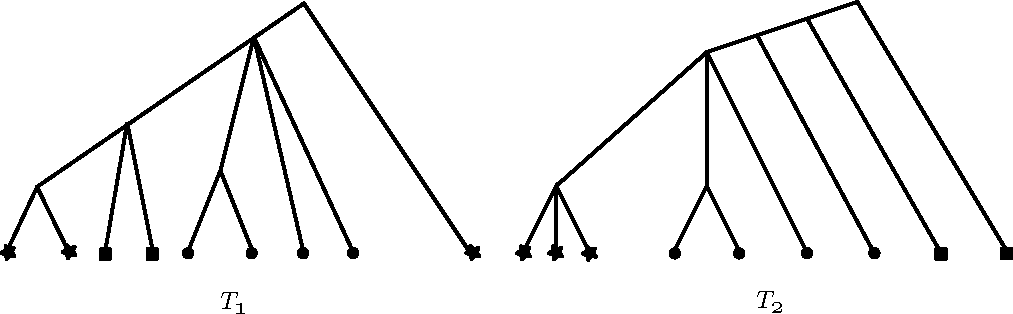
\includegraphics[scale=.8]{../figs/fig_reduc1.pdf}
 \vspace{.5cm}
 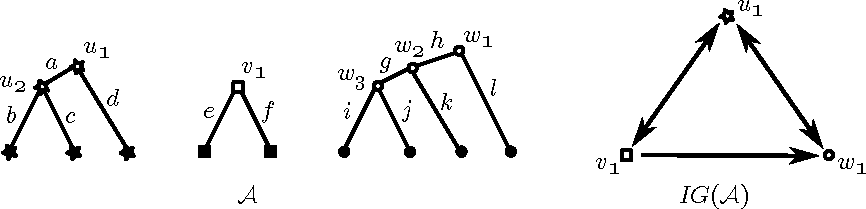
\includegraphics[scale=.9]{../figs/fig_reduc2.pdf}
 \caption{Two trees~$T_1$ and~$T_2$, an agreement forest~$\cA$ for~$T_1$ and~$T_2$ and its inheritance graph $IG(\cA)$. Leaf labels have been omitted.\label{fig:reduc1}}
\end{figure}

\begin{figure}
 \centering
 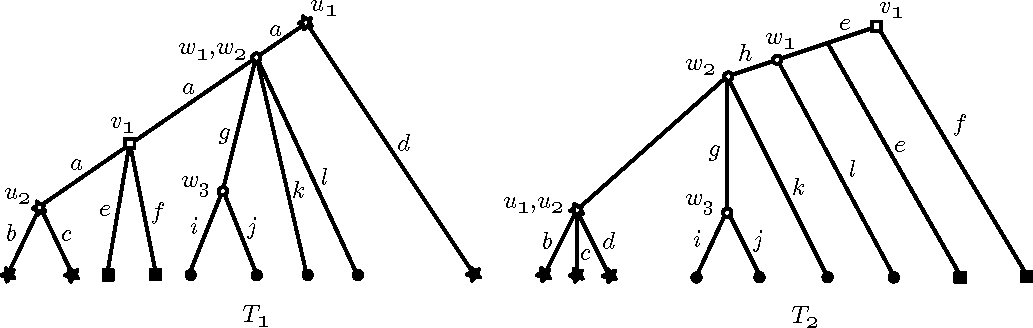
\includegraphics[scale=.8]{../figs/fig_reduc3.pdf}
 \caption{The trees~$T_1$ and~$T_2$ from Figure~\ref{fig:reduc1} labelled with the internal vertices and all edges of~$\cA$.\label{fig:reduc3}}
\end{figure}

\begin{figure}
 \centering
 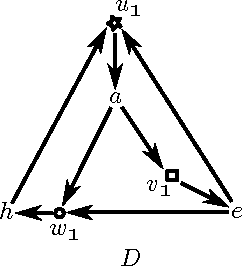
\includegraphics[scale=.9]{../figs/fig_reduc4.pdf}
 \caption{Part of the input graph~$D$ for \dfvs for the trees~$T_1,T_2$ and agreement forest~$\cA$ of Figures~\ref{fig:reduc1} and~\ref{fig:reduc3}. Vertices that do not appear in any directed cycle of~$D$ have been omitted. Minimum feedback vertex sets of~$D$ are $\{u_1\}$ and $\{a\}$.\label{fig:reduc4}}
\end{figure}

From now on, we see an agreement forest as a collection of trees, as specified in the preliminaries section. We can and will assume that the components of~$\cA$ are never more refined than necessary (i.e. there is no agreement forest of~$T_1$ and~$T_2$ that can be obtained from~$\cA$ by contracting edges).

To prepare for the construction of an input graph to \dfvs, we label the vertices and edges of~$T_1$ and~$T_2$ by the vertices and edges of~$\cA$ that they correspond to. Note that each vertex of~$\cA$ is used exactly once as a label but, due to refinements, some vertices of the trees can have multiple labels. Moreover, some edges of~$\cA$ can be used as a label multiple times (when the edge corresponds to a path in a tree) but each edge is used as a label at least once in at least one tree (by the assumption that~$\cA$ is not more refined than necessary). For example, for the trees and agreement forest in Figure~\ref{fig:reduc1}, the labelling is illustrated in Figure~\ref{fig:reduc3}.

We construct an input graph~$D$ for \dfvs as follows. For every internal vertex of $\cA$, we create a vertex for~$D$. Denote the set of these vertices by~$V_V(D)$. In addition, for every edge of~$\cA$ we create a vertex for~$D$. This set of vertices is denoted by~$V_E(D)$. We write $V(D)= V_V(D) \cup V_E(D)$. We create edges of~$D$ as follows. For every $v \in V_V(D)$ and every $e\in V_E(D)$ create an edge $(v,e)$ if $tail(e)=v$ in~$\cA$ and we create an edge $(e,v)$ if~$\hat{v}$ can be reached from $head(\hat{e})$ in at least one tree, for some edge~$\hat{e}$ labelled by~$e$ and the vertex~$\hat{v}$ labelled by~$v$. See Figure~\ref{fig:reduc4} for an example.

We will show that any feedback vertex set of~$D$ corresponds to an $\cA$-splitting and vice-versa. Moreover, after appropriately weighting the vertices of~$D$, the number of ``splits'' of the $\cA$-splitting (i.e. the size of the $\cA$-splitting minus the size of~$\cA$) will be equal to the weight of the corresponding weighted feedback vertex set.

Let~$F\subset V(D)$. In what follows, we use~$F$ both for sets of vertices in~$D$ and for the set of vertices and edges they represent in~$\cA$. Let $\cA \setminus F$ be the forest obtained from~$\cA$ by removing the vertices and edges of~$F$ and repeatedly removing indegree-0 outdegree-1 vertices and suppressing indegree-1 outdegree-1 vertices.

\begin{lemma}
A subset~$F$ of~$V(D)$ is a feedback vertex set of~$D$ if and only if $\cA \setminus F$ is an $\cA$-splitting.
\end{lemma}
\begin{proof}
{Since $F$ can contain only inner vertices of $\cA$} it is clear that $\cA \setminus F$ is an agreement forest of~$T_1$ and~$T_2$. Hence, it is enough to show that $D\setminus F$ has a directed cycle if and only if $IG(\cA \setminus F)$ has a directed cycle.

First, let $C_1, C_2,\ldots, C_k=C_1$ be a cycle in $IG(\cA \setminus F)$. We will show that this implies that there exists a cycle in $D\setminus F$. Let $u_1, u_2,\ldots, u_k$ be the roots of the components $C_1, C_2,\ldots ,C_k$, respectively. Notice that $u_1, u_2,\ldots ,u_k$ are internal vertices of~$\cA$ and hence represented in $D$. Moreover, since these vertices are in $\cA \setminus F$, they are also in $D\setminus F$.

We prove this side of the lemma by showing that the presence of an edge $(C_i, C_{i+1})$ of $IG(\cA \setminus F)$ implies the existence of a directed path from~$u_i$ to~$u_{i+1}$ in $D\setminus F$, for $i=1,\ldots ,k-1$. By the definition of the inheritance graph, an edge $(C_i, C_{i+1})$ of $IG(\cA \setminus F)$ implies that there exists a directed path from~$u_i$ to~$u_{i+1}$ that uses an edge of~$C_i$ in at least one of the trees. It is easy to see that this directed path uses an edge,~$a$ say, of~$C_i$ that has~$u_i$ as its tail. Moreover, since~$C_i$ and~$C_{i+1}$ are components of~$\cA\setminus F$, $u_1,a$ and~$u_{i+1}$ are vertices of $D \setminus F$ and $(u_i,a)$ and $(a,u_{i+1})$ are edges of $D\setminus F$, forming a directed path from~$u_i$ to~$u_{i+1}$ in $D\setminus F$.

Now, assume that $D\setminus F$ contains a cycle. Let $u_1,\ldots,u_k=u_1$ be a longest cycle. We will show that this implies the existence of a cycle in $IG(\cA \setminus F)$. Clearly, $u_1,\ldots ,u_k$ cannot all correspond to vertices and edges from the same component of~$\cA\setminus F$. From the assumption that $u_1,\ldots,u_k=u_1$ is a longest cycle, it can be argued that there are at least two vertices among $u_1,\ldots ,u_k$ that are roots of components of~$\cA\setminus F$. Let $r_1,\ldots ,r_s=r_1$ denote those vertices of the cycle that correspond to roots of components. Let $C_1,\ldots ,C_s$ be the corresponding components of $\cA\setminus F$, respectively. We will show that $C_1,\ldots ,C_s$ form a cycle in $IG(\cA \setminus F)$.

For $i=1,\ldots ,s-1$, we show that there exists an edge $(C_i, C_{i+1})$ in $IG(\cA \setminus F)$. First observe that there exists a directed path from~$r_i$ to~$r_{i+1}$ in $D\setminus F$ and that, since~$D$ is bipartite, this path is of the form
\[
(r_i=v_0, e_1, v_1, e_2, \ldots ,e_t,v_t=r_{i+1})
\]
where $e_1,\ldots ,e_t$ are edges of $\cA \setminus F$ and $v_1,\ldots ,v_{t-1}$ are internal vertices of~$C_i$.

First assume $t=1$. In this case, the path is just $(r_i, e_1,r_{i+1})$. By the definition of~$D$, $tail(e_1)=r_i$ in~$C_i$ and there is a directed path from $head(\hat{e}_1)$ to~$r_{i+1}$, with~$\hat{e}_1$ some edge labelled by~$e_1$, in at least one of the two trees (such an edge $\hat{e}_1$ definitely exists because of the assumption that~$\cA$ is not more refined that necessary). This tree then contains a path from~$r_i$ to~$r_{i+1}$ that contains edge~$\hat{e}_1$ of~$C_i$. Hence there is an edge $(C_i, C_{i+1})$ in $IG(\cA \setminus F)$.

Now assume $t>1$. For~$j=1,\ldots ,t$, by the definition of~$D$, $tail(e_j)=v_{j-1}$ in~$C_i$ and there is a directed path from $head(\hat{e}_j)$ to~$v_j$, with~$\hat{e}_j$ some edge labelled by~$e_j$, in at least one of the two trees. For $j<t$, $e_j$ and~$v_j$ are both in the same component~$C_i$, implying that there is a directed path from $head(e_j)$ to~$v_j$ in~$C_i$. Hence, there is a directed path from~$r_i$ to~$v_{t-1}$ in both trees. Thus, the tree that contains a directed path from~$v_{t-1}$ to~$r_{i+1}$ also contains a directed path from~$r_i$ to~$r_{i+1}$ containing edge~$\hat{e}_t$ of~$C_i$. Hence, $(C_i, C_{i+1})$ is an edge of $IG(\cA \setminus F)$.
\end{proof}

The above lemma showed that we can turn~$\cA$ into an $\cA$-splitting by removing vertices and edges corresponding to a feedback vertex set of~$D$. We will now add weights to the vertices of~$D$ in order to enforce that an optimal feedback vertex set gives an optimal $\cA$-splitting and, moreover, that an approximate feedback vertex set gives an approximate $\cA$-splitting.

We define a weight function~$w$ on vertices of~$D$ as follows, using $\delta^+_\cA(v)$ to denote the outdegree of a vertex~$v$ in~$\cA$.
\begin{displaymath}
  w(v) =
  \begin{cases}
    \delta^+_\cA(v)-1 &\mbox{if } v \in V_V(D)\\
    1 				&\mbox{if } v \in V_E(D).
  \end{cases}
\end{displaymath}

The weight of a feedback vertex set~$F$ is defined as $w(F)= \sum_{v \in F} w(v)$.

Intuitively, the weight of each vertex~$v$ equals the number of components its removal would add to the $\cA$-splitting.

To make this precise, we need the following definition. We call a feedback vertex set~$F$ \emph{proper} if it is minimal (i.e. no proper subset of~$F$ is a feedback vertex set) and if for every vertex~$v\in V_V(D)$ at most $\delta^+_D(v)-2$ children of~$v$ in~$D$ are contained in~$F$, with $\delta^+_D(v)$ denoting the outdegree of~$v$ in~$D$. (Recall that the children of~$v$ in~$D$ are elements of~$V_E(D)$). For example, proper feedback vertex sets of the graph~$D$ in Figure~\ref{fig:reduc4} are $\{u_1\}$ and $\{v_1,w_1\}$. The idea behind this definition is that when all, or all but one, of the children of~$v$ are in~$F$, then we could just as well add~$v$ instead, which does not increase the total weight of the feedback vertex set. Hence, given any feedback vertex set~$F$, a proper feedback vertex set~$F'$ with~$w(F')\leq w(F)$ can be found in polynomial time.

\begin{lemma}
If~$F$ is a proper feedback vertex set of~$D$, then $\cA\setminus F$ is an $\cA$-splitting of size $|\cA| + w(F)$.
\end{lemma}
\begin{proof}
For an edge~$e$ of~$\cA$, we use $tail(e)$ and $head(e)$ to refer to the tail and head of~$e$ in~$\cA$, respectively.

Consider a vertex of~$F$ corresponding to an edge~$e$ of~$\cA$. Then, every cycle in~$D$ that contains~$e$ also contains $tail(e)$. Hence, since~$F$ is minimal, $tail(e)$ is not contained in~$F$. Moreover, suppose that $tail(e)$ is not the root of a component of~$\cA$ and let~$e'$ be the edge with $head(e')=tail(e)$. Then, for every cycle in~$D$ containing~$e$ but not~$e'$ (and hence containing $tail(e)$ but not $tail(e')$), replacing~$e$ and $tail(e)$ by~$e'$ and $tail(e')$ gives again a directed cycle in~$D$. Hence, since~$F$ is minimal, it follows that either~$e'$ or~$tail(e')$ is contained in~$F$, but not both.

Now consider a vertex of~$F$ corresponding to a vertex~$v$ of a component~$C$ of~$\cA$. Then, by the previous paragraph, no edge~$e$ with $tail(e)=v$ is contained in~$F$. Moreover, if~$v$ is not the root of~$C$ and~$e'$ is the edge with $head(e')=v$, then, as before, either~$e'$ or~$tail(e')$ is contained in~$F$, but not both.

To summarize the previous two paragraphs, if~$F$ contains a vertex corresponding to a vertex~$v$ of~$\cA$ that is \emph{not} the root of its component, then~$F$ also contains either the edge entering~$v$ or the parent of~$v$. Similarly, if~$F$ contains a vertex corresponding to an edge~$e$ of~$\cA$ that is \emph{not} leaving the root of its component, then~$F$ also contains either the edge entering~$tail(e)$ or the parent of~$tail(e)$. Informally speaking, this means that if you remove something from a component, you also remove everything above it.

More formally, it follows that $\cA\setminus F$ can be obtained from~$\cA$ by, repeatedly, either removing the root of a component or removing a subset of the edges leaving the root of a component. Moreover, if we remove a subset of the edges leaving the root of a component, at least two of these edges are not removed, because~$F$ is proper.

Removing edges and vertices from~$\cA$ in this way, it is easy to see that the number of components is increased by~$w(F)$.
\end{proof}

To complete the proof of Theorem \ref{thm:maafapprox}, let~$\cA$ be a $c$-approximation to \maf, $F$ a minimal feedback vertex set that is a $d$-approximation to weighted \dfvs on~$D$ and~$F^*$ an optimal  solution to weighted \dfvs on~$D$, then we have:
\begin{align*}
 |\cA\setminus F| - 1 & = |\cA| + w(F) - 1\\
				&\leq |\cA| + d\cdot w(F^*) - 1\\
  				&\leq d(|\cA| + w(F^*) - 1)\\
 				&= d(\mathit{OptSplit}(\cA)-1) \\
 				&\leq d(c+3)\operatorname{MAAF}(T_1,T_2).
\end{align*}

We have thus shown how to construct an agreement forest that is a $d(c+3)$-approximation to \maaf and with that we conclude the proof of Theorem~\ref{thm:maafapprox}.




\section{Experiments} \label{sec:nonbinexp}
%For the nonbinary case, there also exist exact and approximation algorithms for MAF~\cite{nonbinCK,whiddenFixed,whiddenFixedmulti}. In case when one of the input trees is binary we can still use the exact (thus $c=1$) and approximate ($c=3$) algorithms given in \cite{whiddenFixed} (referred to as \textsc{rSPR}) to obtain respectively a 4-approximation and a 6-approximation of the hybridization number problem for nonbinary trees. When both input trees are nonbinary, then we must use the somewhat less optimized exact ($c=1$) and approximate ($c=4$) algorithms described in \cite{nonbinCK}. We then obtain 4- and 7-approximations (because in the nonbinary case $d=1$ is still easily attainable using ILP).

%To measure the approximation ratios attained by \textsc{NonbinaryCycleKiller} in practice we have also implemented and made publicly available the exact nonbinary algorithm \textsc{TerminusEst}, based on the theoretical results in~\cite{terminusest}. \textsc{TerminusEst} will be of independent interest because it is currently the fastest exact nonbinary solver available.

%\Second{\textsc{CycleKiller}, \textsc{NonbinaryCycleKiller} and \textsc{TerminusEst} can be downloaded respectively from \url{http://skelk.sdf-eu.org/cyclekiller} \cite{cyclekillerURL}, from \url{http://homepages.cwi.nl/~iersel/cyclekiller}  \cite{NBCKURL}, and from \url{http://skelk.sdf-eu.org/terminusest} \cite{testURL}}.


To run the simulations with \textsc{NonbinaryCycleKiller}, we used a subset of the trees from the easy set of binary experiments. We then applied random edge contractions in order to obtain nonbinary trees. Hence, we have the same two parameters as before, namely the number of taxa $n \in\{20, 50, 100\}$ and the number of rSPR-moves $k \in \{5, 10, 15, 20\}$, and an additional parameter $\rho \in \{25, 50, 75\}$ which measures the percentage of the edges of an original binary tree that were contracted in order to obtain a nonbinary tree. We could only use smaller values of~$n$ and~$k$ from the easy set of experiments because exact solvers for nonbinary MAF (upon which \textsc{NonbinaryCycleKiller} is built) and exact solvers for nonbinary \textsc{MinimumHybridization} (which is important to measure the accuracy of \textsc{NonbinaryCycleKiller} in practice) are slower than their binary counterparts.

We performed two runs of experiments. One run with instances consisting of one binary and one nonbinary tree, and one run with instances consisting of two nonbinary trees.

For the experiments with one binary and one nonbinary tree, we were still able to use the \textsc{rSPR} algorithm \cite{whiddenRSPRwebsite,whiddenFixed}, which has a better running time and approximation ratio compared to the available algorithm for two nonbinary trees. When \textsc{rSPR} is used in exact mode, \textsc{NonbinaryCycleKiller} yields a theoretical worst-case approximation ratio of 4. When \textsc{rSPR} is used in its 3-approximation mode, \textsc{NonbinaryCycleKiller} yields a theoretical worst-case approximation ratio of 6. %(\Second{see Section \ref{subsecAlgo}}). 
The results of this run are summarized in Table \ref{fig:rspr_for_maf}.

For the experiments with two nonbinary trees, the \textsc{rSPR} software can no longer be used, and instead we used the exact and 4-approximate MAF algorithm described in~\cite{nonbinCK}. This makes \textsc{NonbinaryCycleKiller} behave as a 4-approximation and 7-approximation respectively. %(\Second{see Section \ref{subsecAlgo}}). 
Note that the exact algorithm~\cite{nonbinCK} is considerably slower than \textsc{rSPR}, meaning that in practice \textsc{NonbinaryCycleKiller} struggles with two nonbinary trees more than
when at most one of the trees is nonbinary. The results for this run are summarized in Table~\ref{fig:maf_for_maf}.

The exact hybridization number in both runs was computed by \textsc{TerminusEst}~\cite{testURL}.

Each instance that took longer than~10 minutes to compute was aborted and the running time was set to~600 seconds. The averages of the running-times are taken over all instances, with running-time taken to be~600 if the program timed out for that instance. (We used a shorter time-out than in the binary experiments because of the observation that, in the nonbinary case, exact algorithms running longer than~10 minutes almost always took longer than~60 minutes too.)

Note that we did not compare the performance of \textsc{NonbinaryCycleKiller} to \textsc{Dendroscope} because \textsc{TerminusEst} has better running times than the exact nonbinary \textsc{MinimumHybridization} solver inside \textsc{Dendroscope} (data not shown).

To enable a clearer analysis we divided the trees into representative ``simple'' and ``tricky'' ones based on two parameters,~$n$ and~$k$. Parameter values for the simple set were $n \in \{20, 50\}$, $k \in \{5, 10, 15\}$ and for the tricky set $n \in \{50, 100\}$, $k=20$. In addition we varied the percentage of contracted edges (in a single tree in the first run and in both trees in the second run).


In Table~\ref{fig:rspr_for_maf} we show running times and solution quality of our algorithm when one of the input trees is binary. For the simple set of instances (regardless of the percentage of edge-contractions) we see that the more accurate version of our algorithm, the 4-approximation, had a better running time than the exact algorithm, and at the same time had an average approximation ratio very close to~1. Far more interesting is to see what happens with tricky instances. As predicted, the running time of the exact algorithm is much higher for tricky instances due to the higher hybridization numbers. On the other hand, the running time of the 4-approximation does not rise significantly at all, whilst still attaining an approximation ratio again very close to 1. Another thing to note is that the percentage of contraction only seems to affect the running time of the exact algorithm. The practical worst-case approximation ratio observed in these experiments was~1.75 for the 4-approximation and~3 for the 6-approximation. 


Table \ref{fig:maf_for_maf} shows our results on instances with two nonbinary trees. The exact algorithm for MAF is in this case much slower and this affects the running times even for the simple set. While the 4-approximation version has an average approximation ratio very close to 1 again, the running time is in this case worse than that of \textsc{TerminusEst}. For the tricky set the situation is even more significant; the exact MAF algorithm cannot deal with reticulation numbers above~15, while \textsc{TerminusEst} can get slightly further. On the other hand, the 7-approximation still runs much faster than \textsc{TerminusEst}, both for simple and tricky instances, while having an average approximation ratio of less than 2.6. The practical worst-case approximation ratio observed in these experiments was~1.5 for the 4-approximation and~4 for the 7-approximation. 

%The percentage of contraction in this run seems to affect the running time of the exact algorithm to a larger extent than in the previous run.

%\textcolor{red}{What should we say about that freak of running time for 75 contraction and 4-approximation? I double checked the formula in the spreadsheet and I don't think it is a mistake or a typo...}
It is worth noting that, for the 4-approximation, the running time for the 75\%-contraction trees is considerably lower than the one for the 50\%-contraction trees. This is due to the fact that a high contraction in both trees causes the hybridization number of the instance to drop, and a lower hybridization number leads to a better running time. 
Also note that the exact solver \textsc{TerminusEst} seems more able to cope with the
tricky 25\%-contraction instances than the tricky 50\%-contraction instances. This is probably because, although low contraction rates yield a higher hybridization number, the trees remain ``relatively binary'' and this can induce more efficient branching in the underlying FPT algorithm~\cite{teresaFPT}. It is plausible that with 50\%-contraction the instances suffer from the disadvantage of relatively high hybridization number without the branching advantages associated with (relatively) binary trees.

% To find the limits of the \texttt{7-approx} option of \textsc{NBCK}, we also tested it on huge, biologically meaningless, randomly generated trees. Below some results:
% \begin{itemize}
% \item [$\bullet$]1000 leaves, 25\%-contraction, on average 995 reticulations in 63 sec.
% \item [$\bullet$] 1000 leaves, 50\%-contraction, on average 989 reticulations in 82 sec.
% \item [$\bullet$] 1000 leaves, 75\%-contraction, on average 840 reticulations, in 656 sec. 
% \end{itemize}
% Computation times of this last run of experiments do not include the network construction.
% 
% 


\begin{figure}[h]
	\centering
		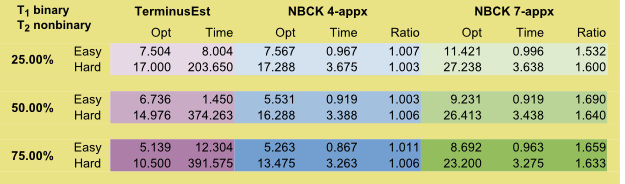
\includegraphics[width=\textwidth]{../figs/table1.png}
	\caption{Summary of results for instances with one binary and one nonbinary tree. We list the average hybridization number found (Opt), the average running time in seconds (Time) and where applicable the average approximation ratio (Ratio) for the three algorithms.}
	\label{fig:rspr_for_maf}
\end{figure}


\begin{figure}[h]
	\centering
		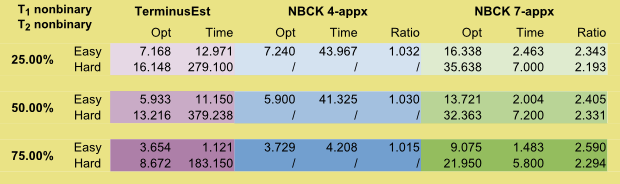
\includegraphics[width=\textwidth]{../figs/table2.png}
	\caption{Summary of results for instances with two nonbinary trees. The layout of the table is the same as that of table \ref{fig:rspr_for_maf}.}
	\label{fig:maf_for_maf}
\end{figure}


%\textcolor{red}{TO DO: make the tables in the same style as in the previous chapter}
% 
% \section{Conclusion}
% We have given improved FPT and polynomial-time approximation algorithms for nonbinary \maf, and demonstrated that, as in the binary case, algorithms for \maf and \dfvs can be combined to yield nontrivial approximation guarantees for nonbinary \maaf. 
% 
% 
% A number of interesting open problems remain. 
% The best known polynomial-time approximation algorithms for both binary and nonbinary \maf have a factor of 3. While for nonbinary \maaf we have shown how to achieve an approximation factor of $d(c+3)$, but for binary the corresponding expression is $d(c+1)$. Might it be that the binary and nonbinary variants of \maaf are equally approximable, or is the nonbinary variant in some sense strictly more difficult to approximate? This gap remains something that needs to be further explored. Our experiments with nonbinary trees highlight once again that the cycle-breaking technique described in this chapter is intrinsically linked to the current state-of-the-art in \textsc{MAF} algorithms. 

%----------------was never a conclusion: -----------------------------
%On the software side, we have implemented both our \maf algorithms and made them publicly available~\cite{mafprogram}. We can report the following provisional performance results. The FPT algorithm solves instances with~$k\leq 14$ within a few minutes. The approximation algorithm solves instances with~$n\leq 500$ within seconds (and possibly larger instances too). The highest approximation-factor encountered on the inputs we tried was~$2.5$ (which raises the question whether the 4-approximation analysis given in this chapter can actually be sharpened). For nonbinary \maaf we have not yet implemented the $d(c+3)$ algorithm but are planning to do so. As in \cite{practicalCycleKiller}, it should be possible to obtain $d=1$ by using Integer Linear Programming (ILP) to solve \dfvs exactly.


% \textsc{TerminusEst} is faster than the most accurate mode of \textsc{NonbinaryCycleKiller} when both trees are nonbinary due to the fact that MAF solvers for two nonbinary trees have not yet been optimized to the same extent as their binary counterparts. In fact, \textsc{TerminusEst} is the best avaible exact method for nonbinary trees and can handle instances for which the optimum is up to~15-20. For other instances, \textsc{NonbinaryCycleKiller} in its fastest mode is much faster than \textsc{TerminusEst} and produces solutions that are at most a factor~4 from the optimum (less than 2.6 on average).
% 
% Finally, for instances with one binary and one nonbinary tree, the most accurate mode of \textsc{NonbinaryCycleKiller} is again much faster than \textsc{TerminusEst} and produces solutions that are at most a factor~1.75 from the optimum (less than 1.011 on average). 
